
\chapter {Architecture of eSim}
\thispagestyle{empty}
\label{chap2}

eSim is a CAD \index{CAD} tool that helps electronic system designers
to design, test and analyse their circuits. But the important feature
of this tool is that it is open source and hence the user can modify
the source as per his/her need. The software provides a generic,
modular and extensible platform for experiment with electronic
circuits. This software runs on Ubuntu Linux LTS distributions 18.04 and 20.04, and  Microsoft Windows 7, 8 and 10.
It uses {\tt Python 3}, {\tt KiCad 4.0.7}, {\tt Makerchip},
{\tt GHDL}, {\tt Verilator} and {\tt Ngspice}.

The objective behind the development of eSim is to provide an open
source EDA solution for electronics and electrical engineers. The 
software should be capable of performing schematic creation, PCB 
design and circuit simulation (analog, digital and mixed-signal). 
It should provide facilities to create new models and components. 
The architecture of eSim has been designed by keeping these 
objectives in mind. 

\section {Modules used in eSim}
Various open-source tools have been used for the underlying build-up 
of eSim. In this section we will give a brief idea about all the modules 
used in eSim. 

\subsection {Eeschema} \index{Eeschema} \index{KiCad}
Eeschema is an integrated software where all functions of circuit
drawing, control, layout, library management and access to the PCB
design software are carried out.  It is the schematic
editor tool used in KiCad. %\cite{eeschema}. 
Eeschema is intended to
work with PCB layout software such as Pcbnew. It provides netlist that
describes the electrical connections of the PCB. Eeschema also
integrates a component editor which allows the creation, editing and
visualization of components. It also allows the user to effectively
handle the symbol libraries i.e; import, export, addition and deletion
of library components.  Eeschema also integrates the following
additional but essential functions needed for a modern schematic
capture software:

\begin{inparaenum}
\item Design rules check \index{Design rules check} ({\tt DRC}) for 
the automatic control of incorrect connections and inputs of components 
left unconnected.
\item Generation of layout files in {\tt POSTSCRIPT} \index{POSTSCRIPT}or 
{\tt HPGL} \index{HPGL} format.
\item Generation of layout files printable via printer.
\item Bill of materials generation.
\item Netlist generation for PCB layout or for simulation.
\end{inparaenum}

This module is indicated by the label 1 in \figref{blockd}.

As Eeschema is originally intended for PCB Design, there are no
fictitious components\footnote{Signal generator or power supply is not
  a single component but in circuit simulation, we consider them as a
  component.  While working with actual circuit, signal generator or
  power supply gives input to the circuit externally thus, doesn't
  require for PCB design.} such as voltage or current sources. Thus,
we have added a new library for different types of voltage and current
sources such as sine, pulse and square wave.  We have also built a
library which gives printing and plotting solutions.
This extension, developed by us for eSim, is indicated by the label
2 in \figref{blockd}.

\subsection {CvPcb}
\index{CvPcb} CvPcb is a tool that allows the user to associate
components in the schematic to component footprints when designing the
printed circuit board. CvPcb is the footprint editor tool in KiCad.
%\cite{eeschema}. 
Typically the netlist file generated by Eeschema does
not specify which printed circuit board footprint is associated with
each component in the schematic. However, this is not always the case
as component footprints can be associated during schematic capture by
setting the component's footprint field. CvPcb provides a convenient
method of associating footprints to components. It provides footprint
list filtering, footprint viewing, and 3D component model viewing to
help ensure that the correct footprint is associated with each
component. Components can be assigned to their corresponding
footprints manually or automatically by creating equivalence
files. Equivalence files are look up tables associating each component
with its footprint. This interactive approach is simpler and less
error prone than directly associating footprints in the schematic
editor.  This is because CvPcb not only allows automatic association,
but also allows to see the list of available footprints and displays
them on the screen to ensure the correct footprint is being
associated.  This module is indicated by the label 3 in
\figref{blockd}.  

\subsection {Pcbnew}
\index{Pcbnew} Pcbnew is a powerful printed circuit board software
tool. It is the layout editor tool used in KiCad. %\cite{eeschema}. 
It
is used in association with the schematic capture software Eeschema,
which provides the netlist. Netlist describes the electrical
connections of the circuit. CvPcb is used to assign each component, in
the netlist produced by Eeschema, to a module that is used by
Pcbnew. The features of Pcbnew are given below:
\begin{itemize}
\item It manages libraries of modules. Each module is a drawing of the
  physical component including its footprint\index{Footprints} - the
  layout of pads providing connections to the component. The required
  modules are automatically loaded during the reading of the netlist
  produced by CvPcb.
\item Pcbnew integrates automatically and immediately any circuit
  modification by removal of any erroneous tracks, addition of 
  new components, or by modifying any value (and under certain
  conditions any reference) of old or new modules, according to
  the electrical connections appearing in the schematic.   
\item This tool provides a rats nest display, a hairline connecting
  the pads of modules connected on the schematic. These
  connections move dynamically as track and module movements are
  made. 
\item It has an active Design Rules Check ({\tt DRC}) which
  automatically indicates any error of track layout in real time. 
\item It automatically generates a copper plane, with or without
  thermal breaks on the pads.  
\item It has a simple but effective auto router to assist in the
  production of the circuit. An export/import in {\tt SPECCTRA}
  dsn format allows to use more advanced
  auto-routers.  
\item It provides options specifically for the production of ultra
  high frequency circuits (such as pads of trapezoidal and complex
  form, automatic layout of coils on the printed circuit).  
\item Pcbnew displays the elements (tracks, pads, texts, drawings and
  more) as actual size and according to personal preferences such as: 
\begin{itemize}
\item display in full or outline.
\item display the track/pad clearance.
\end{itemize}
\end{itemize}
This module is indicated by the label 4 in
\figref{blockd}.
\subsection{KiCad to Ngspice converter}
Analysis parameters, and the source details are provided through this module. It also allows us to add and edit the device models and subcircuits, included in the circuit schematic.  Finally, this module facilitates the conversion of KiCad netlist to Ngspice compatible ones. 
\\
It is developed by us for eSim and it is indicated by the label 7 in \figref{blockd}. The use of this module is explained in detail in section (yet to be put).

%Commenting and putting it in next chapter

%\subsubsection{Analysis Inserter}
%This feature helps the user to perform different types of analysis such
%as Operating point analysis, \index{Operating point analysis} DC
%analysis, \index{DC Analysis} AC analysis, \index{AC Small-signal
%Analysis} transient analysis, \index{Transient Analysis}. It has
%the facility to
%\begin{itemize}
%\item Insert type of analysis such as AC or DC or Transient
%\item Insert values for analysis
%\end{itemize}
%\subsubsection {Source Details}
%eSim sources are added from eSim-sources package. Sources auch as \textit{SINE, AC, DC, PULSE} are in this library. The parameter values to all the sources added in the schematic can be given through 'Source Details'.
%\subsubsection {Ngspice Model}
%Ngspice has in built model such as \textit{flipflop(D,SR,JK,T),gain,summer} etc. which can be utilised while building a circuit.
%eSim allows to add and modify Ngspice model parameter through Ngspice Model tab.
%\subsubsection {Device Modeling}
%Devices like \textit{Diode, JFET, MOSFET, IGBT, MOS} etc added in the circuit can be modeled using device model libraries. eSim also provides editing and adding new model libraries. While converting Kicad to Ngspice these library files are added to the corresponding devices used in the circuit.
%\subsubsection {Subcircuits}
%Subcircuits are the circuits within a circuits. Subcircuiting helps to reuse the part of the circuits.
%The sub circuit in the main circuits are added using this facility. Also, eSim provides us with editing the already existing subcircuits.
%%
\subsection {Model Builder} \index{Model Builder}
This tool provides the facility to define a new model for devices such
as,
\begin{inparaenum}
            \item Diode
            \item Bipolar Junction Transistor (BJT)
            \item Metal Oxide Semiconductor Field Effect Transistor (MOSFET)
            \item Junction Field Effect Transistor (JFET)
            \item IGBT and
            \item Magnetic core.
            \end{inparaenum}
            This module also helps edit existing models.
It is developed by us for eSim and it is indicated by the
label 5 in \figref{blockd}.
 
\subsection{Subcircuit Builder} \index{Subcircuit Builder} This
module allows the user to create a subcircuit for a component. Once
the subcircuit for a component is created, the user can use it in
other circuits. It has the facility to define new components such as,
Op-amps, IC-555, UJT and so on.  This component also helps edit existing
subcircuits.  This module is developed by us for eSim and it is
indicated by the label 6 in \figref{blockd}.

\subsection{Ngspice} \index{Ngspice} \label{sec:ngspice}
Ngspice is a general purpose circuit simulation program for nonlinear
dc, nonlinear transient, and linear ac analysis.
%\cite{ngspice-web}. 
Circuits may contain resistors, capacitors,
inductors, mutual inductors, independent voltage and current sources,
four types of dependent sources, lossless and lossy transmission lines
(two separate implementations), switches, uniform distributed RC
lines, and the five most common semiconductor devices: diodes,
\index{diode} BJTs, \index{BJT} JFETs, MESFETs,
and MOSFET. \index{MOSFET}
This module is indicated by the label 9 in \figref{blockd}.

\subsection{NGHDL} \index{NGHDL} \label{sec:nghdl}
NGHDL, a module for mixed signal circuit simulation, is also integrated with eSim.  It makes use of VHDL code.
It uses ghdl for digital simulation and the mixed signal simulation happens through 
Ngspice.

\subsection{NgVeri} \index{NgVeri} \label{sec:NgVeri}
NgVeri, a module for mixed signal circuit simulation, is also integrated with eSim. It makes use of Verilog/System Verilog/Transaction-Level Verilog  code.
It uses SandPiper SaaS and Verilator for digital simulation and the mixed signal simulation happens through 
Ngspice. 

\subsection{Makerchip-App} \index{Makerchip-App} \label{sec:Makerchip-App}
Makerchip is a cloud based browser application developed by Redwood EDA to do digital circuit design. One can simulate Verilog/SystemVerilog/Transaction-Level Verilog code in Makerchip. eSim is interfaced with Makerchip using a Python based application called Makerchip-App which launches the Makerchip IDE.

\subsection{SandPiper SaaS} \index{SandPiper SaaS} \label{sec:Sandpiper-saas}
Sandpiper-saas is a tool developed by Redwood EDA which converts Transaction Level Verilog code to SystemVerilog code. It is used by NgVeri so that it can get the System Verilog code which can be further passed to the Verilator.

\subsection{Verilator} \index{Verilator} \label{sec:Verilator}
Verilator is a Verilog/SystemVerilog simulator tool. It converts the Verilog/SystemVerilog code to C++ object files. These object files are linked with that of Ngspice thus enabling mixed signal simulation in eSim.

\subsection{OpenModelica} \index{OpenModelica} \label{sec:openmodelica}
OpenModelica (OM) is an open source modeling and simulation tool based on
Modelica language. Two modules of OpenModelica, OMEdit, an IDE for modeling 
and simulation and OMOptim, an IDE for optimisation are integrated with eSim.

\section {Work flow of eSim}

\begin{figure}
\centering
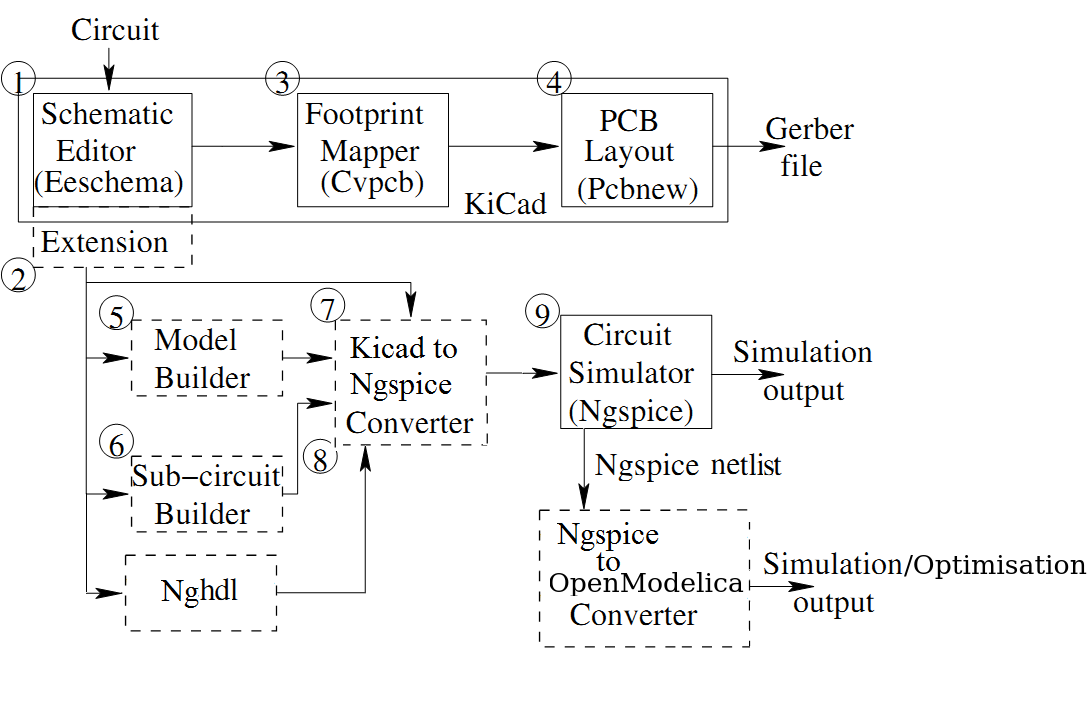
\includegraphics[width=\hgfig]
{blockdiagram.png}
\caption{Work flow in eSim. (Boxes with dotted lines denote
  the modules developed in this work).}
%\caption{Workflow of Oscad}
\label{blockd}
\end{figure}

\figref{blockd} shows the work flow in eSim. The block diagram consists of mainly three parts: 
\begin{itemize}
\item Schematic Editor 
\item PCB Layout Editor  
\item Circuit Simulators
\end{itemize} 



%
Here we explain the role of each block in designing electronic
systems. Circuit design is the first step in the design of an electronic
circuit. Generally a circuit diagram is drawn on a paper, and then
entered into a computer using a schematic editor. Eeschema is the
schematic editor for eSim. Thus all the functionalities of Eeschema
are naturally available in eSim.  \index{EEschema}

Libraries for
components, explicitly or implicitly supported by Ngspice, have been
created using the features of Eeschema. As Eeschema is originally intended for PCB design, there are
no fictitious components such as voltage or current sources. Thus, a
new library for different types of voltage and current sources such as
sine, pulse and square wave, has been added in eSim. A library
which gives the functionality of printing and plotting has also been
created. 

The schematic editor provides a netlist file, which describes the
electrical connections of the  design. In order to create a PCB
layout, physical components are required to be mapped into their
footprints. To perform component to footprint mapping, CvPcb  is
used. Footprints have been created for the
components in the newly created libraries. Pcbnew is used to draw a
PCB layout. 

After designing a circuit, it is essential to check the integrity of
the circuit design. In the case of large electronic circuits,
breadboard testing is impractical. In such cases, electronic system
designers rely heavily on simulation. 
The accuracy of the simulation results can be increased by accurate
modeling of the circuit elements.
Model Builder provides the facility
to define a new model for devices and edit existing models. Complex
circuit elements can be created by hierarchical modeling. Subcircuit
Builder provides an easy way to create a subcircuit. 

The netlist generated by Schematic Editor cannot be directly used
for simulation due to compatibility issues. Netlist Converter converts
it into Ngspice compatible format. The type of simulation
to be performed and the corresponding options are
provided through a graphical user interface (GUI). This is called
KiCad to Ngspice Converter in eSim. 

eSim uses Ngspice for analog, digital, mixed-level/mixed-signal circuit
simulation. Ngspice is based on three open source software
packages%\cite{spice}:  
\begin{itemize}
\item Spice3f5 (analog circuit simulator) 
\item Cider1b1 (couples Spice3f5 circuit simulator to DSIM device simulator)
\item Xspice (code modeling support and simulation of digital components through an event driven algorithm)
\end{itemize}
It is a part of gEDA \index{gEDA} project. Ngspice is capable of
simulating devices with BSIM, \index{BSIM} EKV,  HICUM, \index{EKV}
\index{HICUM} HiSim, \index{HiSim} PSP, \index{PSP} and PTM \index{PTM}
models. It is widely used due to its accuracy even for the latest
technology devices.
